\documentclass[a4paper]{article}

\usepackage[utf8]{inputenc}
\usepackage[polish]{babel}
\usepackage{polski}
\usepackage[margin=0.9in]{geometry}
\usepackage{graphicx}

\author{Aleksandra Grzelak \\* Dorian Janiak \\* Marcin Ochman}
\title{Analizator danych pogodowych}

\begin{document}
\maketitle

\section{Opis}

\section{Diagramy}

Na poniższych rysunkach zostały przedstawione diagramy \textit{ERD} oraz \textit{UML} prezentujące budowę naszej aplikacji.

\begin{figure}[h]
\centering
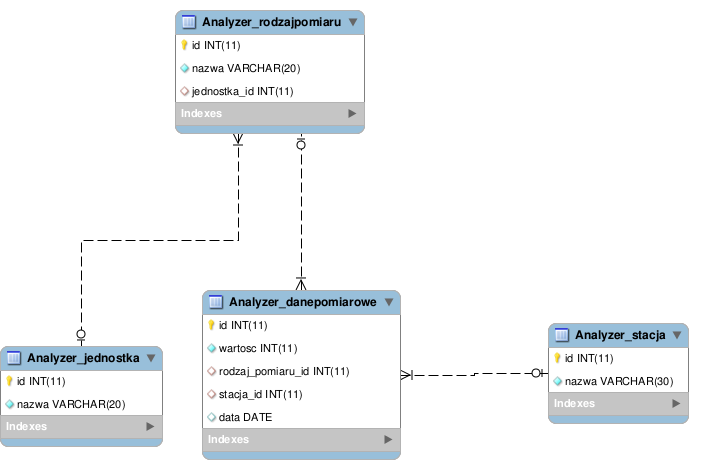
\includegraphics[scale=0.6]{./diagramEER}
\caption{Tabele oraz powiązania pomiędzy nimi w naszej aplikacji}
\label{fig:diagram_eer}
\end{figure}

\begin{figure}[h]
\centering
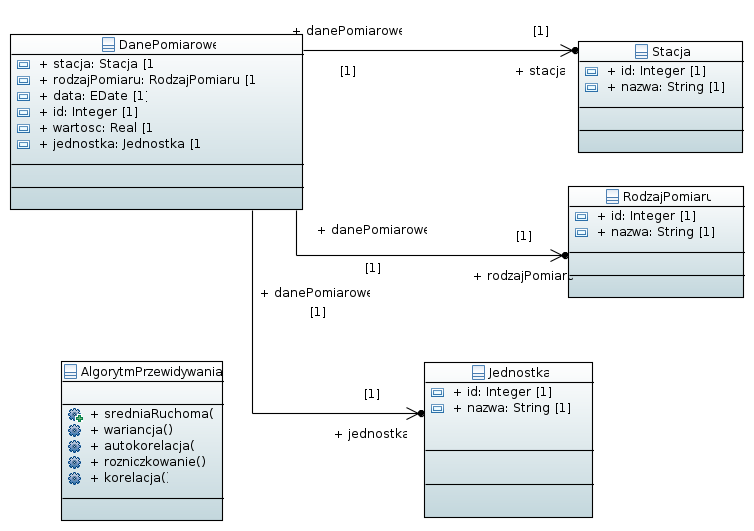
\includegraphics[scale=0.7]{./uml}
\caption{Graficzne przedstawienie klas używanych w aplikacji}
\label{fig:diagram_eer}
\end{figure}

\end{document}